\documentclass[11pt]{scrartcl}
\usepackage{fullpage}

%hype Link:
\usepackage{hyperref}
% Cite
\usepackage{cite}

\usepackage{listings} % Coding Syntax coloring
\usepackage{color}
\usepackage{textcomp}
\definecolor{listinggray}{gray}{0.9}
\definecolor{lbcolor}{rgb}{0.9,0.9,0.9}

\lstset{
     backgroundcolor=\color{lbcolor},
     tabsize=4,
     rulecolor=,
     language=matlab,
        basicstyle=\scriptsize,
        upquote=true,
        aboveskip={1.5\baselineskip},
        columns=fixed,
        showstringspaces=false,
        extendedchars=true,
        breaklines=true,
        prebreak = \raisebox{0ex}[0ex][0ex]{\ensuremath{\hookleftarrow}},
        frame=single,
        showtabs=false,
        showspaces=false,
        showstringspaces=false,
        identifierstyle=\ttfamily,
        keywordstyle=\color[rgb]{0,0,1},
        commentstyle=\color[rgb]{0.133,0.545,0.133},
        stringstyle=\color[rgb]{0.627,0.126,0.941},
}
\usepackage{fancyhdr,graphicx,lastpage}% http://ctan.org/pkg/{fancyhdr,graphicx,lastpage}
\fancypagestyle{plain}{
  \fancyhf{}% Clear header/footer
  \fancyhead[R]{
\includegraphics[scale=0.5]{logo.png}}% Right header
  \fancyhead[L]{\textbf{School of Electronic and Electrical Engineering}}
  %\fancyfoot[L]{Name Firstname - v1.0 \\  Date}% Left footer
  \fancyfoot[R]{\thepage\  / \pageref{LastPage}}% Right footer
}
\pagestyle{plain}% Set page style to plain.


\begin{document}
\title{COMP5880 Assignment 2}
\subtitle{ Scientific Visualization}
\author{Yingjie Luan}
\maketitle

\tableofcontents

\section{Question 1}
We were asked to use draw the isosurfaces for the value G at time 60. The given isovalue is 2500 and 20,000.

\subsection{Code}
See \ref{code:Q1}

\subsection{Generated Images}

\subsubsection{G=2500}
\begin{minipage}[t]{\linewidth}
{
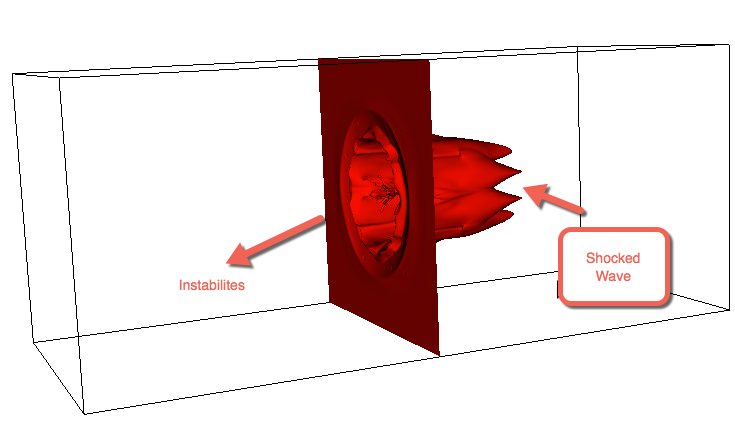
\includegraphics[scale = 0.6]{img_1_2500.png}

\centering
\medskip
{\footnotesize This is the image at $G = 2500$}
}
\end{minipage}

\subsubsection{G=20000}
\begin{minipage}[t]{\linewidth}
{
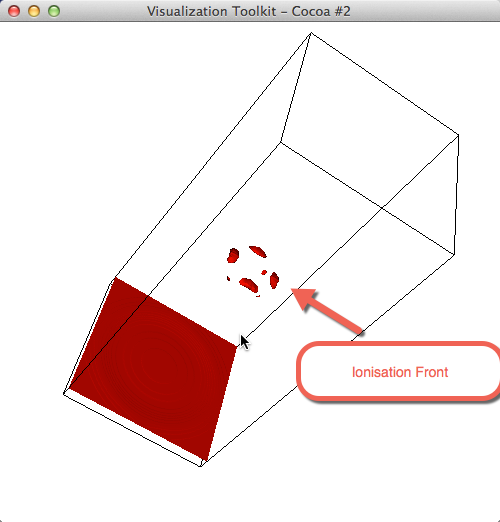
\includegraphics[scale = 0.7]{img_1_20000.png}

\centering
\medskip
{\footnotesize This is the image at $G = 20000$}
}
\end{minipage}

 
\section{Question 2}

We were asked to do a slice for the dataset G at time steps at 45,75 and 135 respectively. 
\subsection{Code}


After tryout, I found that the temperature varies from 70 to 26000, so setting this value as our scalar value will safely guarantee we can cover all the values.\\


We changed the H value as a reference.\\


See \ref{code:Q2} for code.
\subsection{Generated Images}
\subsubsection{Time = 45}
\begin{minipage}[t]{\linewidth}
{
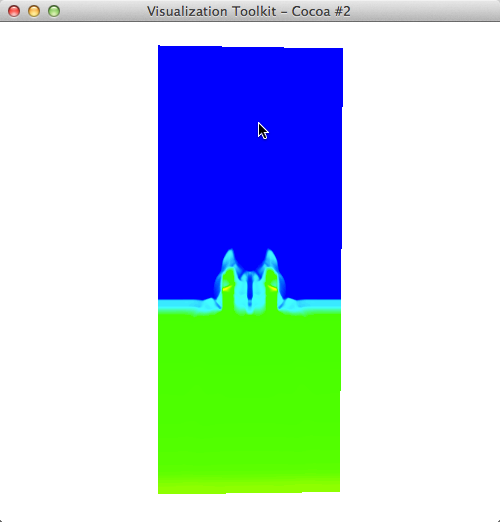
\includegraphics[scale = 0.5]{img_2_45.png}

\centering
\medskip
{\footnotesize This is the image at $T = 45$}
}
\end{minipage}
\subsubsection{Time = 75}
\begin{minipage}[t]{\linewidth}
{
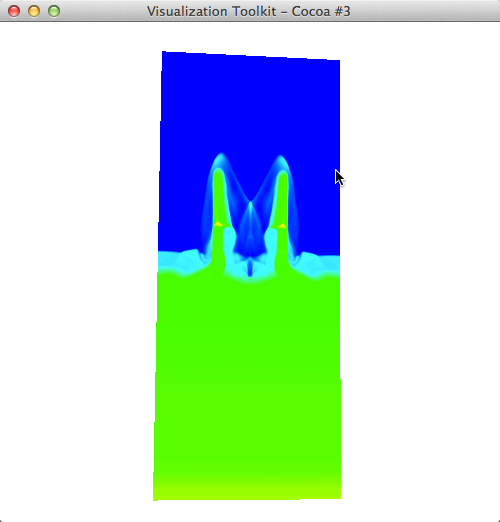
\includegraphics[scale = 0.5]{img_2_75.png}

\centering
\medskip
{\footnotesize This is the image at $T = 75$}
}
\end{minipage}
\subsubsection{Time = 135}
\begin{minipage}[t]{\linewidth}
{
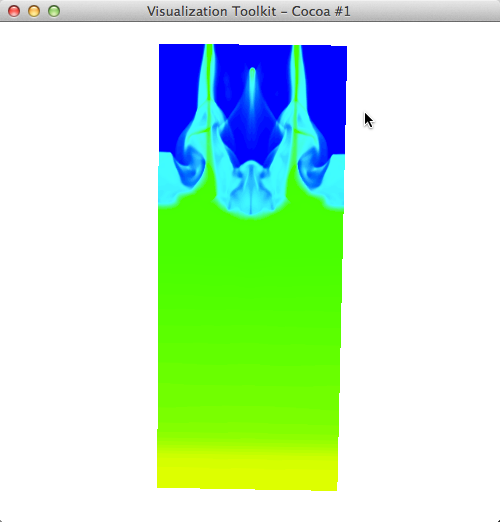
\includegraphics[scale = 0.5]{img_2_135.png}

\centering
\medskip
{\footnotesize This is the image at $T = 135$}
}
\end{minipage}

\section{Question 3}
We were asked to implemented planewidget.
\subsection{Code}
See \ref{code:Q3} for code.

\subsection{Generated Image}
\begin{minipage}[t]{\linewidth}
{
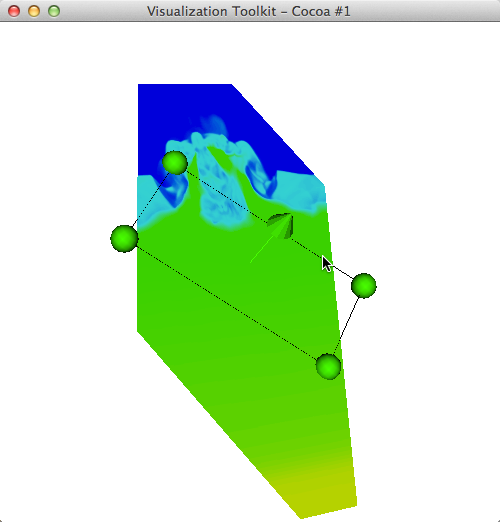
\includegraphics[scale = 0.7]{img_3.png}

\centering
\medskip
{\footnotesize This is the a slice with planewidget. Typing "i" will call or cancel this widget. }
}
\end{minipage}

\section{Question 4}
We were asked to do slice with contour line for the same dataset as Question 2.
\subsection{Code}
See \ref{code:Q4} for code.\\

We changed the color intensity at the HSV schema as a reference for the scalar value.
\subsection{Generated Images}
\subsubsection{Time = 45}
\begin{minipage}[t]{\linewidth}
{
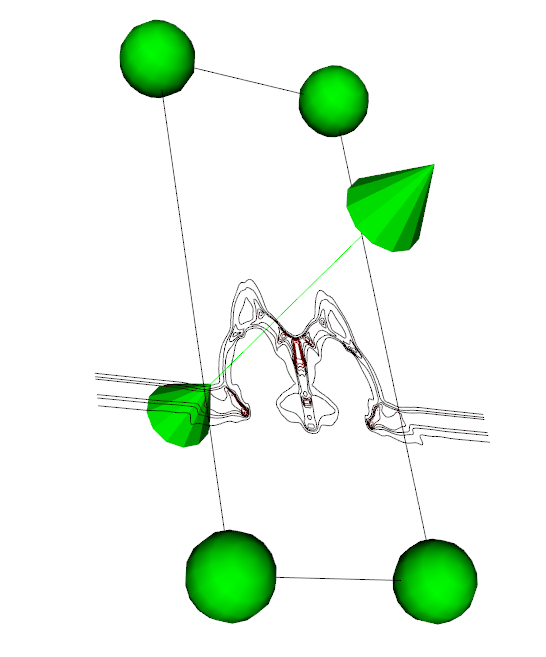
\includegraphics[scale = 0.5]{img_4_45.png}

\centering
\medskip
{\footnotesize This is the image at $T = 45$}
}
\end{minipage}
\subsubsection{Time = 75}
\begin{minipage}[t]{\linewidth}
{
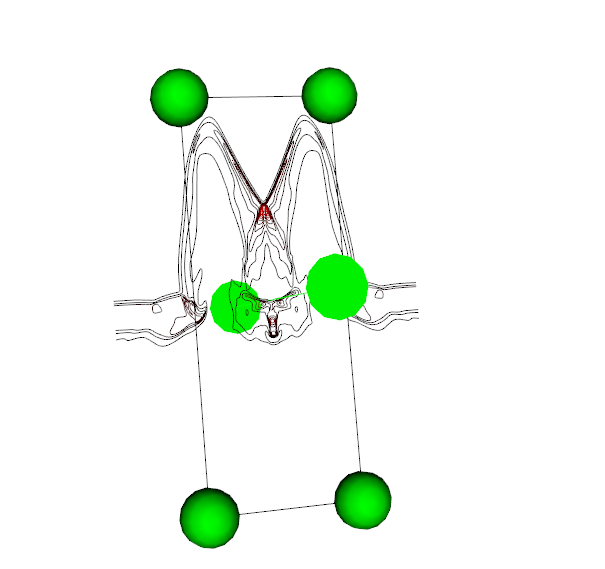
\includegraphics[scale = 0.5]{img_4_75.png}

\centering
\medskip
{\footnotesize This is the image at $T = 75$}
}
\end{minipage}
\subsubsection{Tiem = 135}
\begin{minipage}[t]{\linewidth}
{
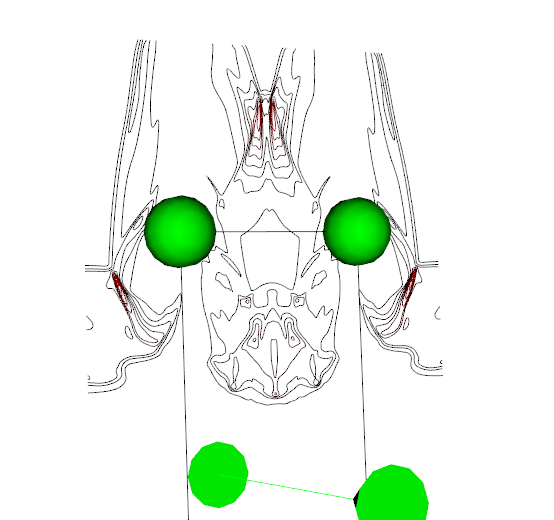
\includegraphics[scale = 0.5]{img_4_135.png}

\centering
\medskip
{\footnotesize This is the image at $T = 135$}
}
\end{minipage}
\section{Question 5}

We were asked to use volume visualization to find the ionisation front and the shockwave at $G = 135$. 

\subsection{Code}

See \ref{code:Q5} for code.\\


\subsection{Generated Image}

By constructing a sharp HSV and a sharp transparency curve I can manage to assign different color according to their values. As we can se, the ionized region located at the two region, where the ionization front is mixed with the shock wave front.\\


\begin{minipage}[t]{\linewidth}
{
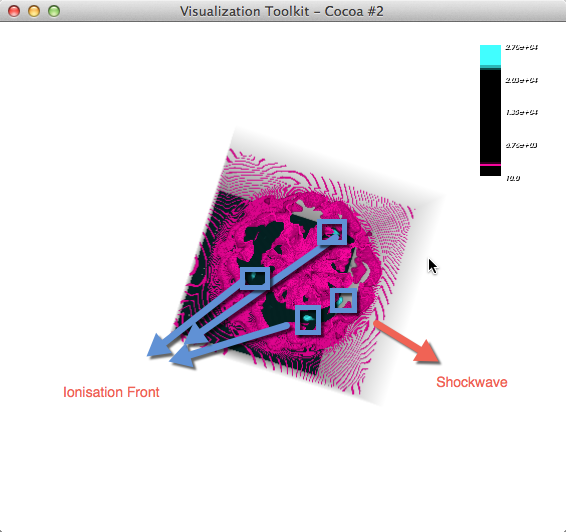
\includegraphics[scale = 0.7]{img_5.png}

\centering
\medskip
{\footnotesize This is the volume visualization. The grey shadow is caused by the unrelated temperature. As we can see, we can find tiny bits of ionisation front within the shockwave.  }
}
\end{minipage}

\section{Question 6}
\subsection{Code}
See \ref{code:Q6} for the code to generate all the screenshots.\\

The way the code is constructed is by overlapping multiply contour and assign each field with distinguishable color.

\subsection{Generated Image}
To relate all the time steps, I generated a screen shot at a fixed position for all the time step and assemble them all together. For animation: \url{http://gifmaker.cc/PlayFrameAnimation.php?folder=2015031222iZwVvaRvkHDLZlz0umLE5Q} \\

\begin{minipage}[t]{\linewidth}
{
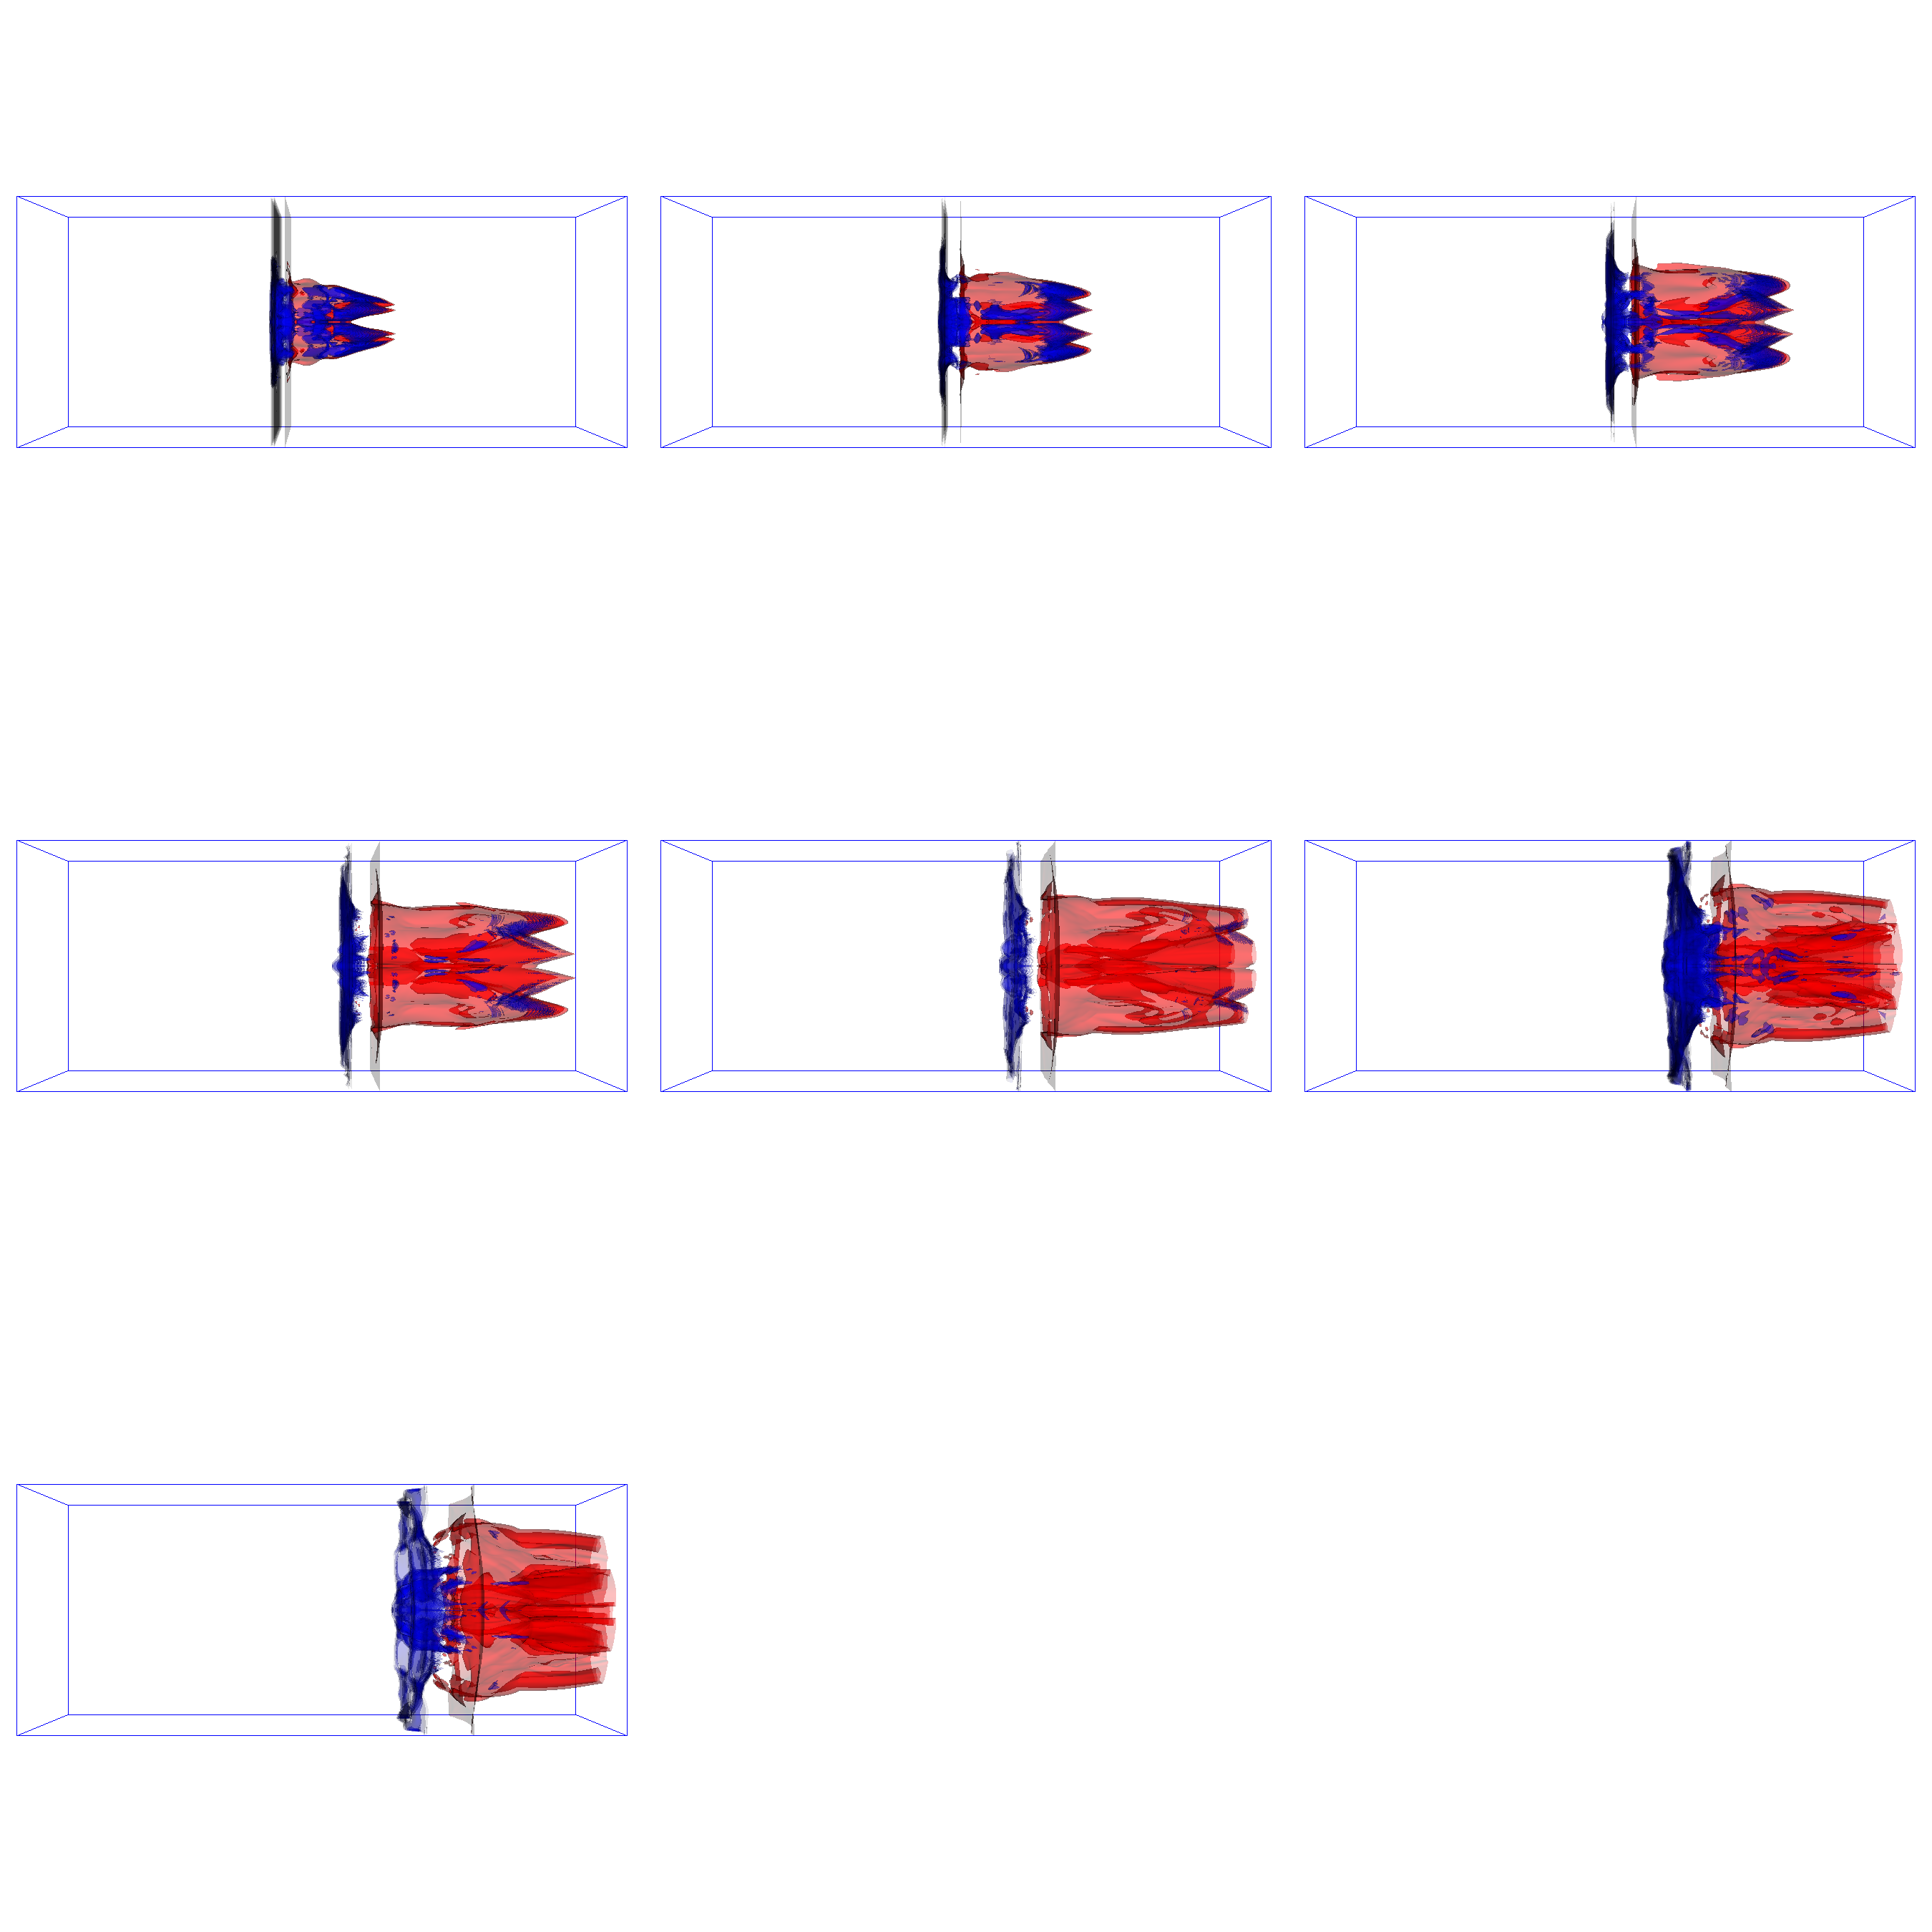
\includegraphics[scale = 0.15]{img_6.png}

\centering
\medskip
{\footnotesize Above are the screenshots at all the time relevant.}
}
\end{minipage}
\subsection{Intention}
According to the \cite[s.~2]{sum2}, the $H_2$ is located at the front of the shockwave. And further, according to the \cite[s.~2,~4]{sum1}, the dissertation points out that $H_2$ is \textit{generated at the very beginning of the ionization process} and \textit{It is most prevalent directly at the beginning of the zone with shocked gas and high turbulence}. So the intention of this visualization is to link the concentration of $H_2$ with G field at value 2500. \\

What's more, according to \cite[s.~4]{sum1}, the distribution of $H_2$ is relatively complex and thus we can ignore the distribution of the total density (D field) and the the distribution of the $H$( H field). That is because \textit{$H_2$ is generated at the very beginning of the cluster, where $H_+$ density is low} and \textit{Very high density of $He_+$, which is greater than 0.15, is observable in the region of $H_2$ formation}.\\

While trying to do so, color mapping was first tried, but due to the difficulty of controlling the color and opacity transfer function, I instead used multiply contour layers. For G field only the shock wave region is showed as a reference($G=2500$). For $H_2$ field, 10 equally separated contour lines was drawn, it starts from the highest $H_2$ value down to the value where $H_2$ is equal to $10\%$ of the highest value.


\subsection{Observation}

As we can see from the animation, at the very beginning of the process, the $H_2$ do concentrate at the front of the shockwave. However, as the time more on, a qualitative change starts to happen. The concentration of $H_2$ begin to trace down and move toward the tail of the shock wave. The highest $H_2$ concentration region has completely shifted to the tail of the shock wave before the shock wave moves out of frame.
\section{Annexes}
\subsection{Q1}
\label{code:Q1}
\begin{lstlisting}[language=Python]
#!/usr/bin/env vtkpython

# Import the VTK library bindings for Python

import vtk

# Create a reader to provide a source for data.
# This filter reads image datasets using VTK's
# XML-based file format.  The file contains
# information about the data format, data
# arrays and extent, so the only parameter that
# the filter needs is the file name.

data = vtk.vtkXMLImageDataReader()
data.SetFileName("/Users/y1275963/Documents/homework/multifield.0060.vti")

data_g = vtk.vtkAssignAttribute()
data_g.SetInputConnection(data.GetOutputPort())
data_g.Assign('G','SCALARS','POINT_DATA')


outline = vtk.vtkOutlineFilter()
outline.SetInputConnection(data_g.GetOutputPort())

outlineMapper = vtk.vtkPolyDataMapper()
outlineMapper.SetInputConnection(outline.GetOutputPort())

outlineActor = vtk.vtkActor()
outlineActor.SetMapper(outlineMapper)
outlineActor.GetProperty().SetColor(0,0,0)


# Create a filter to extract an isosurface from
# the dataset.  Connect the input of this
# filter to the output of the reader.  Set the
# value for the (one) isosurface that we want
# to extract, and tell the filter to compute
# normal vectors for each triangle on the
# output isosurface.

iso = vtk.vtkContourFilter()
iso.SetInputConnection(data_g.GetOutputPort())
iso.ComputeNormalsOn()
iso.SetNumberOfContours(1)
iso.SetValue(0, 20000) #Chnge here to change the isovalue

iso.Update()
outp = iso.GetOutput()
print outp

# Create a mapper to traverse the polydata and
# generate graphics commands for drawing the
# polygons onto the output device.

mapper = vtk.vtkPolyDataMapper()
mapper.SetInputConnection(iso.GetOutputPort())
mapper.ScalarVisibilityOff()

# Output primitives (i.e. the triangles making
# up the isosurface) are managed as an actor;
# we specify that all outputs are coloured
# red.

actor = vtk.vtkActor()
actor.SetMapper(mapper)
actor.GetProperty().SetColor(1, 0, 0)

# Create a renderer which will output the
# graphics commands onto a drawing surface within
# a window.  By default the renderer will fill
# all of the window.  We set the background
# colour of the window to white.

ren1 = vtk.vtkRenderer()
ren1.AddActor(actor)
ren1.AddActor(outlineActor)
ren1.SetBackground(1, 1, 1)#white

# Create the window for output, setting its
# initial size.


renWin = vtk.vtkRenderWindow()
renWin.AddRenderer(ren1)
renWin.SetSize(500, 500)

# Create an interactor to allow mouse and keyboard
# control of the render window content.  VTK supports
# a number of different interaction styles, here we
# choose a "trackball" style where object motion in
# the window starts and stops with input into the
# interaction device.

iren = vtk.vtkRenderWindowInteractor()
iren.SetRenderWindow(renWin)
style = vtk.vtkInteractorStyleTrackballCamera()
iren.SetInteractorStyle(style)

# Initialise the system; this will force the window
# content to be redrawn, triggering execution of the
# visualization pipeline.

iren.Initialize()
iren.Start()
\end{lstlisting}
\subsection{Q2}
\label{code:Q2}
\begin{lstlisting}[language=Python]
# -*- coding: utf-8 -*-
"""
    Created on Fri Mar  6 10:26:23 2015
    
    @author: y1275963
    """
#!/usr/bin/env vtkpython

import vtk

data = vtk.vtkXMLImageDataReader()
data.SetFileName("/Users/y1275963/Documents/homework/multifield.0045.vti")


data_g = vtk.vtkAssignAttribute()
data_g.SetInputConnection(data.GetOutputPort())
data_g.Assign('G','SCALARS','POINT_DATA')

plane = vtk.vtkPlane()
plane.SetOrigin(320, 124, 124)
plane.SetNormal(0, 1, 0)

cut = vtk.vtkCutter()
cut.SetInputConnection(data_g.GetOutputPort())
cut.SetCutFunction(plane)

lut = vtk.vtkLookupTable()
lut.SetNumberOfColors(128)
lut.SetHueRange(0.66,0)
lut.SetValueRange(1,1)
lut.SetSaturationRange(1,1)
lut.Build()

mapper = vtk.vtkPolyDataMapper()
mapper.SetInputConnection(cut.GetOutputPort())
mapper.SetScalarRange(72,26000)
mapper.SetLookupTable(lut)
mapper.SetColorModeToMapScalars()

actor = vtk.vtkActor()
actor.SetMapper(mapper)

ren1 = vtk.vtkRenderer()
ren1.SetBackground(1, 1, 1)
ren1.AddActor(actor)

renWin = vtk.vtkRenderWindow()
renWin.AddRenderer(ren1)
renWin.SetSize(500, 500)

iren = vtk.vtkRenderWindowInteractor()
iren.SetRenderWindow(renWin)

style = vtk.vtkInteractorStyleTrackballCamera()
iren.SetInteractorStyle(style)

iren.Initialize()
iren.Start()
\end{lstlisting}
\subsection{Q3}
\label{code:Q3}
\begin{lstlisting}[language=Python]
# -*- coding: utf-8 -*-
"""
    Created on Fri Mar  6 10:26:23 2015
    
    @author: y1275963
    """
#!/usr/bin/env vtkpython

import vtk

data = vtk.vtkXMLImageDataReader()
data.SetFileName("/Users/y1275963/Documents/homework/multifield.0135.vti")


data_g = vtk.vtkAssignAttribute()
data_g.SetInputConnection(data.GetOutputPort())
data_g.Assign('G','SCALARS','POINT_DATA')

# Create planewidget
planeWidget = vtk.vtkPlaneWidget()
planeWidget.SetInput(data_g.GetOutput())
planeWidget.NormalToZAxisOn()
planeWidget.SetResolution(20)
planeWidget.SetRepresentationToOutline()
planeWidget.PlaceWidget([0,640, 0,248, 0,248])
planeWidget.SetHandleSize(planeWidget.GetHandleSize() * 0.5)
planeWidget.GetPlaneProperty().SetColor(0,0,0)
planeWidget.GetHandleProperty().SetColor(0,1,0)

plane = vtk.vtkPlane()
planeWidget.GetPlane(plane)

# Cutting
cut = vtk.vtkCutter()
cut.SetInputConnection(data_g.GetOutputPort())
cut.SetCutFunction(plane)

lut = vtk.vtkLookupTable()
lut.SetNumberOfColors(121248)
lut.SetHueRange(0.66,0)
lut.SetValueRange(1,1)
lut.SetSaturationRange(1,1)
lut.Build()

mapper = vtk.vtkPolyDataMapper()
mapper.SetInputConnection(cut.GetOutputPort())
mapper.SetScalarRange(72,33000)
mapper.SetLookupTable(lut)
mapper.SetColorModeToMapScalars()

actor = vtk.vtkActor()
actor.SetMapper(mapper)

ren1 = vtk.vtkRenderer()
ren1.SetBackground(1, 1, 1)
ren1.AddActor(actor)

renWin = vtk.vtkRenderWindow()
renWin.AddRenderer(ren1)
renWin.SetSize(500, 500)

iren = vtk.vtkRenderWindowInteractor()
iren.SetRenderWindow(renWin)

style = vtk.vtkInteractorStyleTrackballCamera()
iren.SetInteractorStyle(style)


def Start(obj, event):
    global plane, actor
    obj.GetPlane(plane)
    actor.VisibilityOn()

def UpdatePlane(obj, event):
    global plane
    obj.GetPlane(plane)

planeWidget.SetInteractor(iren)
planeWidget.AddObserver("EnableEvent", Start)
planeWidget.AddObserver("InteractionEvent", UpdatePlane)   
    
style = vtk.vtkInteractorStyleTrackballCamera()
iren.SetInteractorStyle(style)

iren.Initialize()
iren.Start()
\end{lstlisting}
\subsection{Q4}
\label{code:Q4}
\begin{lstlisting}[language=Python]
#!/usr/bin/env vtkpython

import vtk

data = vtk.vtkXMLImageDataReader()
data.SetFileName("/Users/y1275963/Documents/homework/multifield.0135.vti")

data_g = vtk.vtkAssignAttribute()
data_g.SetInputConnection(data.GetOutputPort())
data_g.Assign('G','SCALARS','POINT_DATA')

plane = vtk.vtkPlane()
plane.SetOrigin(320, 124, 124)
plane.SetNormal(0, 1, 0)


cut = vtk.vtkCutter()
cut.SetInputConnection(data_g.GetOutputPort())
cut.SetCutFunction(plane)

iso = vtk.vtkContourFilter()
iso.SetInputConnection(cut.GetOutputPort())
#iso.SetNumberOfContours(8)
iso.GenerateValues(16, 72, 26000)

lut = vtk.vtkLookupTable()
lut.SetNumberOfColors(64)
lut.SetHueRange(1,1)
lut.SetValueRange(0.5,1)
lut.SetSaturationRange(1,1)
lut.Build()

mapper = vtk.vtkPolyDataMapper()
mapper.SetInputConnection(iso.GetOutputPort())
mapper.SetScalarRange(72,26000)
mapper.SetLookupTable(lut)
mapper.SetColorModeToMapScalars()

actor = vtk.vtkActor()
actor.SetMapper(mapper)

ren1 = vtk.vtkRenderer()
ren1.SetBackground(1, 1, 1)
ren1.AddActor(actor)

renWin = vtk.vtkRenderWindow()
renWin.AddRenderer(ren1)
renWin.SetSize(500, 500)

iren = vtk.vtkRenderWindowInteractor()
iren.SetRenderWindow(renWin)

style = vtk.vtkInteractorStyleTrackballCamera()
iren.SetInteractorStyle(style)

iren.Initialize()
iren.Start()
\end{lstlisting}

\subsection{Q5}
\label{code:Q5}
\begin{lstlisting}[language=Python]
# -*- coding: utf-8 -*-
"""
    Created on Fri Mar  6 10:26:23 2015
    
    @author: y1275963
    """
#!/usr/bin/env vtkpython

import vtk

data = vtk.vtkXMLImageDataReader()
data.SetFileName("/Users/y1275963/Documents/homework/multifield.0135.vti")


data_g = vtk.vtkAssignAttribute()
data_g.SetInputConnection(data.GetOutputPort())
data_g.Assign('G','SCALARS','POINT_DATA')

opacityTransferFunction = vtk.vtkPiecewiseFunction()
opacityTransferFunction.AddPoint(10.0, 0.001)
opacityTransferFunction.AddPoint(1900.0,0.001 )
opacityTransferFunction.AddPoint(2000.0, 1.0)
opacityTransferFunction.AddPoint(2500.0, 1.0)
opacityTransferFunction.AddPoint(2600.0, 0.001)
opacityTransferFunction.AddPoint(22000.0, 0.001)
opacityTransferFunction.AddPoint(23000.0, 1.0)
opacityTransferFunction.AddPoint(27000.0, 1.0)

colorTransferFunction = vtk.vtkColorTransferFunction()
colorTransferFunction.AddHSVPoint(10.0, 0.1, 0.0, 0.0)
colorTransferFunction.AddHSVPoint(1900.0, 0.1, 0.0, 0.0)
colorTransferFunction.AddHSVPoint(2000.0, 0.9, 1.0, 1.0)
colorTransferFunction.AddHSVPoint(2500.0, 0.9, 1.0, 1.0)
colorTransferFunction.AddHSVPoint(2600.0, 0.6, 0.0, 0.0)
colorTransferFunction.AddHSVPoint(22000.0, 0.6, 0.0, 0.0)
colorTransferFunction.AddHSVPoint(23000.0, 0.5, 1.0, 1.0)
colorTransferFunction.AddHSVPoint(27000.0, 0.5, 1.0, 1.0)

volumeProperty = vtk.vtkVolumeProperty()
volumeProperty.SetColor(colorTransferFunction)
volumeProperty.SetScalarOpacity(opacityTransferFunction)
volumeProperty.SetInterpolationTypeToLinear()
volumeProperty.ShadeOff()

#compositeFunction = vtk.vtkVolumeRayCastCompositeFunction()
volumeMapper = vtk.vtkFixedPointVolumeRayCastMapper()
#volumeMapper.SetFixedPointVolumeRayCastFunction(compositeFunction)
volumeMapper.SetInputConnection(data_g.GetOutputPort())
volumeMapper.SetBlendModeToComposite()



## Adding ScalarBar:
scalarBar = vtk.vtkScalarBarActor()
scalarBar.SetLookupTable(colorTransferFunction)
scalarBar.SetOrientationToVertical()
scalarBar.SetPosition( 0.85, 0.7 );
scalarBar.SetPosition2( 0.1, 0.3 );

volume = vtk.vtkVolume()
volume.SetMapper(volumeMapper)
volume.SetProperty(volumeProperty)

ren1 = vtk.vtkRenderer()
ren1.SetBackground(1, 1, 1)
ren1.AddVolume(volume)
ren1.AddActor(scalarBar)


renWin = vtk.vtkRenderWindow()
renWin.AddRenderer(ren1)
renWin.SetSize(500, 500)

iren = vtk.vtkRenderWindowInteractor()
iren.SetRenderWindow(renWin)

style = vtk.vtkInteractorStyleTrackballCamera()
iren.SetInteractorStyle(style)

iren.Initialize()
iren.Start()
\end{lstlisting}
\subsection{Q6}
\label{code:Q6}
\begin{lstlisting}[language=Python]
# -*- coding: utf-8 -*-
"""
Created on Fri Mar 13 10:15:51 2015

@author: y1275963
"""

#!/usr/bin/env vtkpython

# Import the VTK library bindings for Python

import vtk
def contour_G(filename):
    # Creating contour for G fileld
    
    data = vtk.vtkXMLImageDataReader()
    data.SetFileName(filename)     

    data_g = vtk.vtkAssignAttribute()
    data_g.SetInputConnection(data.GetOutputPort())
    data_g.Assign('G','SCALARS','POINT_DATA')
    

    outline = vtk.vtkOutlineFilter()
    outline.SetInputConnection(data_g.GetOutputPort())
    
    outlineMapper = vtk.vtkPolyDataMapper()
    outlineMapper.SetInputConnection(outline.GetOutputPort())
    
    outlineActor = vtk.vtkActor()
    outlineActor.SetMapper(outlineMapper)
    outlineActor.GetProperty().SetColor(0,0,1)
    
    
    iso = vtk.vtkContourFilter()
    iso.SetInputConnection(data_g.GetOutputPort())
    iso.ComputeNormalsOn()
    iso.SetNumberOfContours(1)
    iso.SetValue(0, 2500) #Chnge here to change the isovalue
    
    
    mapper = vtk.vtkPolyDataMapper()
    mapper.SetInputConnection(iso.GetOutputPort())
    mapper.ScalarVisibilityOff()
    
  
    actor = vtk.vtkActor()
    actor.SetMapper(mapper)
    actor.GetProperty().SetColor(1, 0, 0)
    actor.GetProperty().SetOpacity(0.5)
    
 
    return (outlineActor,actor)
def multi_con_h2(filename):
    # Creating contour for h2 fileld
    
    data = vtk.vtkXMLImageDataReader()
    data.SetFileName(filename) 
    data.Update()
    #Getting highest value
    [low,high] = data.GetOutput().GetPointData().GetArray("H2").GetRange()

    data_h2 = vtk.vtkAssignAttribute()
    data_h2.SetInputConnection(data.GetOutputPort())
    data_h2.Assign('H2','SCALARS','POINT_DATA')
    
    
    
 
    iso = vtk.vtkContourFilter()
    iso.SetInputConnection(data_h2.GetOutputPort())
    iso.ComputeNormalsOn()
    iso.SetNumberOfContours(10)
    for i in range(10):
        iso.SetValue(i, (1.0-0.1*i)*high) #Chnge here to change the isovalue
    
    
 
    
    mapper = vtk.vtkPolyDataMapper()
    mapper.SetInputConnection(iso.GetOutputPort())
    mapper.ScalarVisibilityOff()
    
 
    
    actor = vtk.vtkActor()
    actor.SetMapper(mapper)
    actor.GetProperty().SetColor(0, 0, 1)
    actor.GetProperty().SetOpacity(0.3)
    
 
    return actor

 
def single_graph(filename):
    outlineActor_G,actor_G = contour_G(filename)
    actor_h2 = multi_con_h2(filename)
    ren1 = vtk.vtkRenderer()
    ren1.AddActor(actor_G)
    ren1.AddActor(actor_h2)
    ren1.AddActor(outlineActor_G)
    ren1.SetBackground(1, 1, 1)#white
    
 
    return ren1
def create_img(path,filename):
    ren1 = single_graph(path+filename+".vti")
    renWin = vtk.vtkRenderWindow()
     
    renWin.SetOffScreenRendering(1)
    renWin.AddRenderer(ren1)

    renWin.Render()
    
    windowToImageFilter = vtk.vtkWindowToImageFilter()
    windowToImageFilter.SetInput(renWin)
    windowToImageFilter.SetMagnification(3)
    windowToImageFilter.SetInputBufferTypeToRGBA()
    windowToImageFilter.ReadFrontBufferOff()
    windowToImageFilter.Update()
    
    writer = vtk.vtkPNGWriter()
    writer.SetFileName(filename+".png")
    writer.SetInputConnection(windowToImageFilter.GetOutputPort())
    writer.Write()
if __name__ == "__main__":
    create_img("/Users/y1275963/Documents/homework/","multifield.0045")
    create_img("/Users/y1275963/Documents/homework/","multifield.0060")
    create_img("/Users/y1275963/Documents/homework/","multifield.0075")
    create_img("/Users/y1275963/Documents/homework/","multifield.0090")
    create_img("/Users/y1275963/Documents/homework/","multifield.0105")
    create_img("/Users/y1275963/Documents/homework/","multifield.0120")
    create_img("/Users/y1275963/Documents/homework/","multifield.0135")
\end{lstlisting}


\bibliographystyle{plain}
\bibliography{bibliography}
\end{document}